\documentclass[9pt,a4paper,twoside]{../rho-class/rho}
\usepackage{ctex}
\usepackage{amsmath}
\usepackage{amssymb}
\usepackage{siunitx}
\usepackage{hyperref}
\usepackage{indentfirst}
\usepackage{fontspec}
\usepackage{esint}

\setCJKmainfont{Noto Serif CJK SC}
\setsansfont{Noto Sans CJK SC}

\setCJKmainfont{Noto Serif CJK SC}[BoldFont=Noto Sans CJK SC,ItalicFont=LXGW WenKai]

\setbool{rho-abstract}{true} % Set false to hide the abstract
\setbool{corres-info}{false} % Set false to hide the corresponding author section
\setbool{linenumbers}{false} % Set false to hide the line numbering

\renewcommand{\vec}{\overrightarrow}

\sisetup{
    mode = math, 
    reset-math-version = false, 
}
\setlength{\parindent}{2em}
\linespread{1.2}

%----------------------------------------------------------
% TITLE
%----------------------------------------------------------

\journalname{电磁学 A \ 课程论文}
\title{不可定向曲面上的 Gauss 定理推广}

%----------------------------------------------------------
% AUTHORS AND AFFILIATIONS
%----------------------------------------------------------

% \author[1,$\dagger$]{崔俊熙}
% \author[2,$\ddagger$]{实验主管老师}
% \author[2,$\ddagger$]{实验助教}
\author{崔俊熙 PB25000124}

%----------------------------------------------------------

% \affil[1]{中国科学技术大学少年班学院}
% \affil[2]{中国科学技术大学物理学院}
% \affil[$\dagger$]{学号: PB25000124.}
% \affil[$\ddagger$]{实验指导教师.}

%----------------------------------------------------------
% DATES
%----------------------------------------------------------

% \dates{本篇实验报告收稿于2026年XX月XX日，于2026年XX月XX日提交.}
\dates{2026-XX-XX}

%----------------------------------------------------------
% FOOTER INFORMATION
%----------------------------------------------------------

\leadauthor{崔俊熙 PB25000124}
\footinfo{电磁学 A \ 课程论文}
\smalltitle{不可定向曲面上的 Gauss 定理推广}
\institution{中国科学技术大学}
\theday{\today}

%----------------------------------------------------------
% ARTICLE INFORMATION
%----------------------------------------------------------

% \corres{Provide the corresponding author information and publisher here.}
\email{cuijunxi@mail.ustc.edu.cn.}

% \received{March 20, 2024}
% \revised{April 16, 2024}
% \accepted{April 20, 2024}
% \published{May 21, 2024}

% \license{Rho LaTeX Class \ccLogo\ This document is licensed under Creative Commons CC BY 4.0.}

\hypersetup{
    pdftitle={不可定向曲面上的 Gauss 定理推广},
    pdfauthor={崔俊熙},
    pdfsubject={电磁学A 课程论文},
    pdfcreator={LaTeX},
    pdfproducer={XeLaTeX}
}

%----------------------------------------------------------
% ABSTRACT
%----------------------------------------------------------

\begin{abstract}
    在这里写摘要 XXXXXX
\end{abstract}

%----------------------------------------------------------

\keywords{ 关键词 XXX; XXXX; XXXXX}

%----------------------------------------------------------

\begin{document}

\maketitle
\thispagestyle{firststyle}
% \tableofcontents

%----------------------------------------------------------

\section{引言} \label{sec:introduction}
\rhostart{在}

\section{可定向曲面} \label{sec:orientable-surfaces}

\subsection{可定向曲面通量} \label{subsec:orientable-surface-flux}

我们想研究不可定向曲面上类似 Gauss 定理的性质, 而起失去了定向性.
故 Gauss 定理不能完全直接用在其上, 必然失去一些信息.
我们要讨论哪些信息可以保留. 在迁移前我们先在\textbf{可定向曲面}中进一步研究.

我们定义一个映射 $E: S^2 \to \bbR^3$, 让 $S^2$ 上每一点 $p$ 对应至该处场 $\vec{E} = E(p)$.

我们再具体化一点, 对于这个映射值域 $E(S^2) \subseteq \bbR^3$, 由于 $S^2$ 是面,
则 $E(S^2)$ 只会是点, 线, 面, 而不会是体, $\bbR^3$ 中许多冗余. 我们需要造一个面容纳 $E(S^2)$, 记为 $F$.
我们定义另一个映射 $f: S^2 \to F$, 仍有 $S^2$ 上一点 $P$,
对应至 $\vec{E} = E(p) = f(p) \in E(S^2) \subseteq F$, 以此优化这个冗余.

首先考虑一个标准球面 $S^2: x^2 + y^2 + z^2 = r^2$, 处于球心有一个正 (负) 点电荷, 与匀强电场三种情形.

\begin{description}
    \item[Case 1 球心有一个正电荷:]
        此时电场 $E: r \vec{e_r} \to \frac{1}{4 \pi \varepsilon_0} \frac{q}{r^2} \vec{e_r}$,
        则 $E(r \vec{e_r}) \propto \vec{e_r}$,
        即其值域为一个半径为 $\frac{1}{4 \pi \varepsilon_0} \frac{q}{r^2}$ 的球面 $F$.
        每一点处电场强度均为 $F$ 上与该点同向的点 (所表示的向量).
        此时映射 $f: r \vec{e_r} \to \frac{1}{4 \pi \varepsilon_0} \frac{q}{r^2} \vec{e_r}$ 为 $S^2$ 与 $F$ 的一一映射, 没有冗余.

        我们考察其通量
        \[ \Phi = \oiint_{S^2} \vec{E} \cdot \dif \vec{S} = \oiint_{S^2} f \cdot \dif \vec{S} = \oiint_{S^2} \delta \lrvert{f} \lrvert{\dif \vec{S}} \]
        $\delta$ 为关于面元 $\dif \vec{S}$ 位置的函数, 取值为 $[-1, 1]$, 表征 $f$ 与 $\dif \vec{S}$ 间方向关系.
        在这种情况下,
        \[ q = \varepsilon_0 \Phi = \varepsilon_0 \oiint_{S^2} \delta \lrvert{f} \lrvert{\dif \vec{S}} = \varepsilon \lrvert{E} \oiint_{S^2} \delta \dif \vec{S} \]
        当然我们知道 $\delta \equiv 1, q = -4 \pi \varepsilon_0 r^2 \lrvert{E}$.

    \item[Case 2 球心处有一个负电荷:]
        此时电场 $E: r \vec{e_r} \to \frac{1}{4 \pi \varepsilon_0} \frac{q}{r^2} \vec{e_r}$,
        则 $E(r \vec{e_r}) \propto -\vec{e_r}$,
        即其值域为一个半径为 $\frac{1}{4 \pi \varepsilon_0} \frac{q}{r^2}$ 的球面 $F$.
        每一点处电场强度均为 $F$ 上与该点反向的点 (所表示的向量).
        此时映射 $f: r \vec{e_r} \to \frac{1}{4 \pi \varepsilon_0} \frac{q}{r^2} \vec{e_r}$,
        $\delta \equiv -1$, $Q = -4 \pi \varepsilon_0 r^2 \lrvert{E}$.
    
    \item[Case 3 匀强电场:]
        空间中电场均为 $\vec{E_0} = (E_{0x}, E_{0y}, E_{0z})$, 则 $E \equiv E_0$ 为常映射.
        它把球面上每一点都对应到 $(E_{0x}, E_{0y}, E_{0z})$ 这一个点,
        我们把它放在 $x^2 + y^2 + z^2 = \lrvert{\vec{E_0}}^2$ 的球面 $F$ 上看.
        \[ f: S^2 \to F, f(p) = (E_{0x}, E_{0y}, E_{0z}) \]
        此时只有一点 $\delta = 1$, 只有一点 $\delta = -1$, 其余 $\delta = 0$.
        故 $q = \varepsilon_0 \lrvert{E_0} \oiint_{S^2} \delta \dif \vec{S} = 0$.
\end{description}

\subsection{手性与特化通量} \label{subsec:chirality-and-specialized-flux}

\subsubsection{三角分割与定向曲面} \label{subsubsec:triangular-partitioning-and-orientable-surfaces}

球作为一个闭曲面, 其封闭性使研究复杂. 我们想将其分割成闭曲面, 使其两两交于边界, 再研究局部性质.

对于 $S^2$ 我们取其四点

\begin{table}{cc}
    A(0, 0, r) & B(\frac{2\sqrt{2}}{3} r, 0, -\frac{1}{3} r) \\
    C(-\frac{\sqrt{2}}{3} r, \frac{\sqrt{6}}{3} r, -\frac{1}{3} r) & D(-\frac{\sqrt{2}}{3} r, -\frac{\sqrt{6}}{3} r, -\frac{1}{3} r)
\end{table}

取平面 $OAB, OBC, OCA, OCD , ODA, OCA, OBD$ 与圆相交的劣弧将其分割为四个带边闭曲面 $\Omega_A, \Omega_B, \Omega_C, \Omega_D$.
其中, $\Omega_A$ 指 $A$ 相对的那个.

对于一个平面 $ABC$, 单位法向量有两个方向 (穿透纸面向内或向外), 记为 $[ABC]$ 与 $[ACB]$, 且 $[ABC] = [BCA] = [CAB]$,
其中 $[ABC]$是指 $\vec{AB}, \vec{BC}, \vec{CA}$ 呈右手法则的那一个,
同时称 $[AB] = \vec{AB}, [BC] = \vec{BC}, [CA] = \vec{CA}$ 为 $[ABC]$ 所诱导的方向,
同样 $[ACB]$ 诱导方向 $[AC], [CB], [BA]$.

对于曲面 (比如 $\Omega_A$) 它自身是可定向的, 故我们用法向量场代替法向量, $A$ 到 $B$ 有向曲线代替 $\vec{AB}$.
可将该概念推广, 我们称两个曲面的定向相容, 指它们没有公共边界, 或定向在公共边界上分别诱导的定向相反.
称一个曲面可定向, 是指它的所有三角分割, 可取一个定向, 使之两两相容.

比如球面可定向, 是因为 $\Omega_A, \Omega_B, \Omega_C, \Omega_D$ 都可取向球外的那个定向, 这组定向是相容的,
并且我们默认对球的分割的单形的定向即为指向球外的那个, 记为 $[\Omega_A], [\Omega_B], [\Omega_C], [\Omega_D]$.

\subsubsection{$\delta$ 与手性} \label{subsubsec:delta-and-chirality}

我们想研究 \ref{subsec:orientable-surface-flux} 节中几个情况下 $\delta$ 与其所处局部的关系,
如果延长 $OA, OB, OC, OD$ 交 

\begin{rhoenv}[frametitle=注意.]
    注意事项注意事项注意事项注意事项注意事项注意事项注意事项注意事项注意事项注意事项注意事项注意事项注意事项注意事项注意事项
\end{rhoenv}



如果需要插入图片，可以参考
\begin{figure}[H]
    \centering
    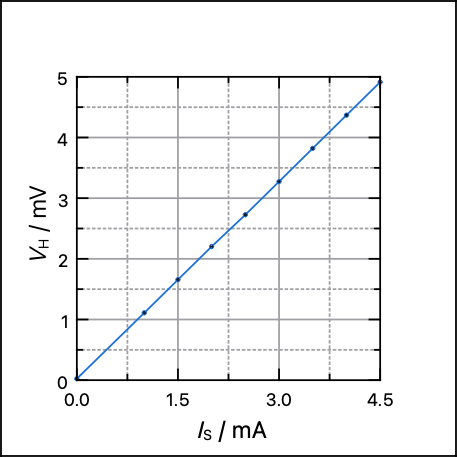
\includegraphics[width=0.72\columnwidth]{1.png}
    \caption{固定励磁电流 $I_M=0.45$ A不变时，绘制得$V_H$-$I_S$ 的关系图线.}
\end{figure}


\end{document}